%--------------------------------------------------------------------------------------
% Definition of the document
%--------------------------------------------------------------------------------------
\documentclass[12pt]{article}
%--------------------------------------------------------------------------------------
% Define packages needed for the writing
%--------------------------------------------------------------------------------------
% General document formatting
\usepackage[margin=1in]{geometry}
%\usepackage[parfill]{parskip}
\usepackage[utf8]{inputenc}    
% Related to math
\usepackage{amsmath,amssymb,amsfonts,amsthm}
% To write derivative more efficiently
\usepackage{physics}
% To add figures
\usepackage{graphicx}
%--------------------------------------------------------------------------------------
% Define the specific setup for the document
% --------------------------------------------------------------------------------------
\newtheorem{theorem}{Theorem}[section]
\theoremstyle{definition}
\newtheorem{definition}{Definition}[section]
\newtheorem{corollary}{Corollary}[theorem]
\theoremstyle{remark}
\newtheorem*{remark}{Remark}
%--------------------------------------------------------------------------------------
% Define the specific setup for the document
%--------------------------------------------------------------------------------------
% Set the font of the equations to Helvetica as well. 
% Increase the spacing between the lines
\linespread{1.5}
% Set the graphics-path, i.e. where we store the figures
\graphicspath{{./images/}}
%--------------------------------------------------------------------------------------
% THE DOCUMENTS BEGINS
%--------------------------------------------------------------------------------------
\begin{document}
\title{\textbf{Fibre-preserving symmetries of time-invariant models in mathematical biology acting on the phase plane}}
\author{Johannes Borgqvist}
\date{\today}
\maketitle
\tableofcontents
\clearpage
%--------------------------------------------------------------------------------------
% THE INTRO
\section{Introduction}
There are numerous examples of biological systems that give rise to oscillatory behaviour. Some of these are the dynamics of a population consisting of predators and prey, chemical reactions such as the Belusov-Zhabotinskii reaction or the so called Brusselator reaction proposed by Prigogene and Lefever. In these cases, the oscillations have been modelled by mathematical models consisting of a two state system of first order ODEs describing the change in either populations sizes or the concentrations of chemical species over time. Mathematically, these oscillations have been described in terms of linear stability analysis, where the models are firstly linearised around their steady states and then the stability of these local linear systems is determined. However, this analytical tool can merely answer questions about the long term behaviour of the system and it does not reveal what properties that are conserved during these oscillations.

A well-known mathematical technique for deriving conserved properties in theoretical physics is that of symmetry methods. Symmetries are transformations which preserve the defining property of the objects they act on, and in the context of ODEs a symmetry is an operator mapping a solution curve to another solution curve. Moreover, symmetries have been used with huge success in theoretical physics to describe physical entities in terms of conservation laws. Here, we aim to apply these techniques on oscillatory dynamical systems modelled by a two state system of first order ODEs. In particular, we will focus on three models, namely the Lotka-Volterra (LV) model, the SIR model sometimes referred to as the Kermack-McKendrick model, the Belusov-Zhabotinskii (BZ) model and the so called Brusselator. The (dimensionless) LV model is given by 

\begin{equation}
  \begin{split}
    \dv{u}{\tau}&=u(1-v),\\
    \dv{v}{\tau}&=\alpha v(u-1).\\    
    \end{split}
  \label{eq:LV}
\end{equation}
and it describes the ``predator-prey'' dynamics of the evolution of prey $u(\tau)$ and predators $v(\tau)$ at dimensionless time $\tau$. The SIR-model is given by describes the dynamics of the spread of an epidemic in a population consisting of susceptibles $S(t)$, infectives $I(t)$ and the removed class $R(t)$. The model is given by
\begin{equation}
  \begin{split}
    \dv{S}{t}&=-rSI,\\
    \dv{I}{t}&=rSI-aI,\\
    \dv{R}{t}&=aI,\\
    \end{split}
  \label{eq:SIR}
\end{equation}
where $r>0$ is the infection rate and $a>0$ is the removal rate of infectives. Moreover, the BZ model is given by

\begin{equation}
  \begin{split}
    \dv{u}{\tau}&=\dfrac{1}{\varepsilon}v-\dfrac{1}{\varepsilon}\left(\dfrac{1}{3}u^3-u\right),\\
    \dv{v}{\tau}&=-u.\\    
    \end{split}
  \label{eq:BZ}
\end{equation}
describing the formation and degradation of the two chemical species $u(\tau)$ and $v(\tau)$ at time $\tau$. Similarly, another oscillatory chemical system is the so called Brusselator given by

\begin{equation}
  \begin{split}
    \dv{u}{\tau}&=1-(b-1)u+au^2 v,\\
    \dv{v}{\tau}&=bu-au^2 v.\\
    \end{split}
  \label{eq:Brusselator}
\end{equation}
where $u(\tau)$ and $v(\tau)$ are two chemical species. All these three systems can give rise to oscillatory behaviour, and our aim of this work is to be able to characterise oscillations in two state dynamical systems of first order ODEs in terms of their symmetries. Inspired by these three systems, we will restrict our focus to \textit{autonomous} systems, specifically \textit{time-invariant} systems, where the right hand sides are given by polynomials in the states $u$ and $v$. For these type of systems, it is well-known that oscillations correspond to closed trajectories in the $(u,v)$-phase plane and therefore we will furthermore restrict our analysis to symmetries that act exclusively on the $(u,v)$-phase plane meaning that these symmetries are independent of time. Subsequently, we will derive the general equation defining fibre-preserving symmetries restricted to the $(u,v)$-phase plane, after that we will present the symmetries of each of these models and lastly we will interpret their meaning by deriving the differential invariants associated with these symmetries. 



%--------------------------------------------------------------------------------------
%--------------------------------------------------------------------------------------
% Fibre preserving symmetries
\section{Mathematical theory of symmetries of differential equations}
Here, we will present a condensed version of the mathematical theory of symmetries of differential equations. For the interested reader, there are many excellent introductory texts~\cite{bluman1989symmetries,hydon2000symmetry,olver2000applications,olver2008equivalence,lang2001,nakahara2003} and here we will focus on general two component of first order ODEs

\begin{equation}
  \begin{split}
    \dv{u}{\tau}&=\omega_1(t,u,v),\\
    \dv{v}{\tau}&=\omega_2(t,u,v),\\    
    \end{split}
  \label{eq:sys_general}
\end{equation}
describing the time evolution of either the concentration profile of two proteins $u(\tau)$ and $v(\tau)$ or the evolution of two populations. Given this system, we subsequently will present the notions of Lie-transformations, their prolongations and symmetries of differential equations. 


% Lie groups of infinitesimal transformations
\subsection{Lie groups of infinitesimal transformations}
Here, a one parameter Lie-symmetry meaning a one parameter $\mathcal{C}^{\infty}$-diffeomorphism is a transformation
\begin{equation}
  (\hat{\tau}(t,u(\tau),v(\tau);\epsilon),\hat{u}(t,u(\tau),v(\tau);\epsilon),\hat{v}(t,u(\tau),v(\tau);\epsilon))=\left(\phi_1(\tau,u,v;\epsilon),\phi_2(\tau,u,v;\epsilon),\phi_3(\tau,u,v;\epsilon)\right)
  \label{eq:symmetry_original}
  \end{equation}
parameterised by the parameter $\epsilon$ where the transformation is defined by the infinitely differentiable functions $\phi_i\in\mathcal{C}^{\infty}(\mathbb{R}^4),\quad i=1,2,3$. Now, we will parametrise such symmetries in terms of $\epsilon$ in the following way
\begin{equation}
\Gamma_{\epsilon}:(\tau,u(\tau),v(\tau))\mapsto\left(\hat{\tau}(\epsilon),\hat{u}(\epsilon),\hat{v}(\epsilon)\right)
\label{eq:symmetry_general}
\end{equation}
and the characterising feature of a symmetry of a differential equation is that if $(\tau,u(\tau),v(\tau))$ is a solution to the system of ODEs in Equation \eqref{eq:sys_general} then so is $(\hat{\tau}(\epsilon),\hat{u}(\epsilon),\hat{v}(\epsilon))$. The set of such one parameter Lie-transformations $G$ together with a multiplication operation $\times$, forms a \textit{one parameter Lie group of transformations} denoted by $(G,\times)$. Such a Lie-group has three defining properties:

\begin{enumerate}
    \item \textit{Multiplication}: For two transformation parameters $\epsilon,\delta\in\mathbb{R}$, multiplication of symmetries (meaning that we first transform with $\delta$ and then with $\epsilon$) is defined by: $\Gamma_\epsilon\times\Gamma_\delta=\Gamma_{\epsilon+\delta}$,
    \item \textit{Identity element}: The trivial symmetry $\Gamma_0=\Gamma_{\epsilon=0}$ acts trivially on curves: $\Gamma_0 (\tau,u(\tau),v(\tau))=(\tau,u(\tau),v(\tau))$,
    \item \textit{Inverse element}: The inverse symmetry $\Gamma^{-1}_{\epsilon}$ is defined by $\Gamma^{-1}_{\epsilon}=\Gamma_{-\epsilon}$.
\end{enumerate}
Moreover, by the continuity of these transformations we can Taylor expand $\Gamma_{\epsilon}$ around $\epsilon\approx 0$ which gives us
\begin{align}
  \hat{\tau}&=\tau+\xi(\tau,u,v)\epsilon+\mathcal{O}(\epsilon^2),\\
  \hat{u}&=u+\eta_1(\tau,u,v)\epsilon+\mathcal{O}(\epsilon^2),\\
  \hat{v}&=v+\eta_2(\tau,u,v)\epsilon+\mathcal{O}(\epsilon^2),
\end{align}
and here the tangents $\xi$, $\eta_1$ and $\eta_2$ are referred to as the \textit{infinitesimals} which, in turn, are defined as follows:
\begin{align}
  \xi(\tau,u,v)&=\left.\pdv{\phi_1(\tau,u,v;\epsilon)}{\epsilon}\right|_{\epsilon=0},\label{eq:tangent_1}\\
  \eta_1(\tau,u,v)&=\left.\pdv{\phi_2(\tau,u,v;\epsilon)}{\epsilon}\right|_{\epsilon=0},\label{eq:tangent_2}\\
  \eta_2(\tau,u,v)&=\left.\pdv{\phi_3(\tau,u,v;\epsilon)}{\epsilon}\right|_{\epsilon=0},\label{eq:tangent_3}
\end{align}
where the functions $\phi_1,\phi_2,\phi_3\in\mathcal{C}^{\infty}(\mathbb{R}^{4})$ define the symmetry according to Equation \eqref{eq:symmetry_original}. Now, one of the most powerful results from the theory of Lie-symmetries is that the global behaviour of the symmetry in Equation \eqref{eq:symmetry_general} can be retrieved from the local behaviour in terms of the infinitesimals in Equations \eqref{eq:tangent_1} to \eqref{eq:tangent_3}. More precisely, the vector field defined by
\begin{equation}
X=\xi(\tau,u,v)\partial_t+\eta_1(\tau,u,v)\partial_u+\eta_2(\tau,u,v)\partial_v
  \label{eq:generator}
\end{equation}
is referred to as the \textit{infinitesimal generator of the Lie group}. Using this vector field, \textit{Lie's first fundamental theorem} \cite{bluman1989symmetries} says that the symmetry in Equation \eqref{eq:symmetry_general}, is in fact given by

\begin{equation}
\Gamma_{\epsilon}:(\tau,u,v)\mapsto \left(e^{\epsilon X}\tau,e^{\epsilon X}u,e^{\epsilon X}v\right)
  \label{eq:symmetry_Lie}
\end{equation}
where the exponential map is defined as follows
\begin{equation}
  e^{\epsilon X}=\sum_{j=0}^{\infty}\dfrac{\epsilon^j}{j!}X^{j}.
  \label{eq:exponential}
\end{equation}
Accordingly, it is enough to know the local behaviour represented by the infinitesimal generator of the Lie group $X$ in Equation \eqref{eq:generator} in order to also know the global behaviour of the symmetry according to Equation \eqref{eq:symmetry_Lie}. Thus, to find the symmetries we must find the infinitesimals which is possible owing to the fact that the defining property of symmetries can be expressed in terms of their local action. Before, we are able to present the notion of a symmetry of a differential equation, we must introduce the idea of so called extended transformations or prolongations.






% Prolongations: extended transformations
\subsection{Prolongations: extended transformations}
Our aim is to mathematically define a symmetry of a differential equation as a Lie-transformation that maps a solution curve of the differential equation to another solution curve. More precisely, given the Lie transformation
$$\Gamma_{\epsilon}:(\tau,u(\tau),v(\tau))\mapsto(\hat{t}(\epsilon),\hat{u}(\epsilon),\hat{v}(\epsilon))$$
we would say that $\Gamma_\epsilon$ is a symmetry of the system of differential equations in Equation \eqref{eq:sys_general} if it maps a solutions curve $(\tau,u(\tau),v(\tau))$ of this system of ODEs to another solution curve $(\hat{t}(\epsilon),\hat{u}(\epsilon),\hat{v}(\epsilon))$. Here, $\tau\in\mathcal{B}\sim\mathbb{R}$ is called the \textit{independent variable} and it defines the so called \textit{base space} $\mathcal{B}$ of the symmetry $\Gamma_\epsilon$. Also, the states $(u(\tau),v(\tau))\in F\sim\mathbb{R}^2$ are called the \textit{dependent variables} and they define the so called \textit{fibre} $F$ of the symmetry $\Gamma_\epsilon$. Given these spaces, the symmetry $\Gamma_\epsilon$ acts on the so called \textit{total space} $E$ defined as $E=B\times F\sim\mathbb{R}^3$, and thus we have that $\Gamma_\epsilon:E\mapsto E$. Now, a transformation acting on solutions to differential equations must account for the derivatives of the states, e.g. $u'(\tau)$ and $v'(\tau)$, and to this end we introduce the notion of extended transforamtions.

There is a natural extension of a Lie-symmetry $\Gamma_\epsilon$ referred to as the prolongation of the symmetry and it is defined by the derivatives of the states. More precisely, \textit{the first prolongation of the Lie-symmetry} $\Gamma^{(1)}_{\epsilon}$ is defined as follows
\begin{equation}
\Gamma_{\epsilon}^{(1)}:(\tau,u(\tau),v(\tau),u'(\tau),v'(\tau))\mapsto(\hat{t}(\epsilon),\hat{u}(\epsilon),\hat{v}(\epsilon),\hat{u}'(\epsilon),\hat{v}'(\epsilon))
  \label{eq:prolongation}
\end{equation}
where the derivatives of the states are defined by $u'(\tau)=\omega_1(t,u,v)$ and $v'(\tau)=\omega_1(t,u,v)$ according to Equation \eqref{eq:sys_general}. Here, it is not entirely clear how the derivatives $\hat{u}'(\epsilon)$ and $\hat{v}'(\epsilon)$ are defined, and to this end we need to introduce the notion of the \textit{total derivative} $D_\tau$. This operator is defined as follows

\begin{equation}
D_\tau=\partial_\tau+u'(\tau)\partial_u+v'(\tau)\partial_v
  \label{eq:tot_der}
  \end{equation}
  and given the total derivative the derivatives of the transformed coordinates are defined as follows
  \begin{equation}
    \begin{split}
      \hat{u}'(\epsilon)&=\dfrac{D_\tau \hat{u}(\tau,u,v;\epsilon)}{D_\tau\hat{\tau}(\tau,u,v;\epsilon)},\\
      \hat{v}'(\epsilon)&=\dfrac{D_\tau \hat{v}(\tau,u,v;\epsilon)}{D_\tau\hat{\tau}(\tau,u,v;\epsilon)}.\\
    \end{split}
    \label{eq:extended_derivatives}
    \end{equation}
    Moreover, the derivatives $(u'(\tau),v'(\tau))\in F'\sim\mathbb{R}^2$ define the \textit{prolonged fibre} $F'$, and \textit{the first jet space} $\mathcal{J}^{(1)}$ is defined by $\mathcal{J}^{(1)}=E\times F'$. Given the jet space, the prolonged symmetry can be succintly written in the following way $\Gamma^{(1)}_{\epsilon}:\mathcal{J}^{(1)}\mapsto\mathcal{J}^{(1)}$. Also, the operator $\Gamma_\epsilon\mapsto\Gamma^{(1)}_{\epsilon}$ is well-defined and is referred to as the \textit{lift} of the symmetry $\Gamma_{\epsilon}$. Previously, we showed that the infinitesimal action of the symmetry $\Gamma_{\epsilon}$ is expressed by the infinitesimal generator of the Lie group $X$ in Equation \eqref{eq:generator}, and similarly there is an infinitesimal representation of the prolonged symmetry $\Gamma^{(1)}_{\epsilon}$.

    Locally, we can describe the action of the first prolongation of the symmetry $\Gamma^{(1)}_{\epsilon}$ by the \textit{first prolongation of the infinitesimal generator of the Lie group} $X^{(1)}$. This operator is defined as follows
\begin{equation}
X^{(1)}=X+\eta_1^{(1)}(\tau,u,v)\partial_{u'}+\eta_2^{(1)}(\tau,u,v)\partial_{v'}
\label{eq:prolonged_generator}
\end{equation}
and here the prolonged infinitesimals $\eta_1^{(1)}$ and $\eta_{2}^{(1)}$ respectively are given by the \textit{prolongation formula}
\begin{equation}
\eta_{i}^{(1)}(\tau,u,v)=D_\tau\eta_i(\tau,u,v)-\omega_i(\tau,u,v) D_\tau\xi(\tau,u,v),\quad i=1,2.
  \label{eq:prolongation_formula}
\end{equation}
Now, given the notion of prolongations, we are now able to formulate the conditions that define a symmetry of a differential equation. 


% Lie symmetries of differential 
\subsection{Symmetries of differential equations}
Consider a one parameter Lie transformation $\Gamma_\epsilon:(\tau,u(\tau),v(\tau))\mapsto(\hat{\tau}(\epsilon),\hat{u}(\epsilon),\hat{v}(\epsilon))$. Then, this transformation is a symmetry of the system of differential equations in Equation \eqref{eq:sys_general} if it maps a solution curve $(\tau,u(\tau),v(\tau))$ to another solution curve $(\hat{\tau}(\epsilon),\hat{u}(\epsilon),\hat{v}(\epsilon))$. Using the notions of jet spaces and prolongations, it can be shown that a Lie-transformation $\Gamma_\epsilon$ is a symmetry of the system of differential equations in Equation \eqref{eq:sys_general} if and only if the following so called \textit{symmetry conditions} hold
\begin{equation}
 \begin{split}
   u'(\epsilon)&=\omega_1(\hat{\tau}(\epsilon),\hat{u}(\epsilon),\hat{v}(\epsilon))\quad\mathrm{whenever}\quad\dv{u}{\tau}=\omega_1(\tau,u,v),\\
   v'(\epsilon)&=\omega_2(\hat{\tau}(\epsilon),\hat{u}(\epsilon),\hat{v}(\epsilon))\quad\mathrm{whenever}\quad\dv{v}{\tau}=\omega_2(\tau,u,v),\\   
 \end{split}
 \label{eq:sym_cond}
\end{equation}
where the derivatives $u'(\epsilon)$ and $v'(\epsilon)$ are defined by Equation \eqref{eq:extended_derivatives}. In general, it is difficult to use these symmetry conditions and instead one can formulate the same condition in terms of the infinitesimal action of the prolonged symmetry. 



 More precsely, a Lie transformation $\Gamma_\epsilon$ is a symmetry of the system of differential equations in Equation \eqref{eq:sys_general} if and only if the \textit{linearised symmetry conditions} given by
\begin{equation}
  \begin{split}
    X^{(1)}\left(\dv{u}{\tau}-\omega_1(\tau,u,v)\right)&=0\quad\mathrm{whenever}\quad\dv{u}{\tau}=\omega_1(\tau,u,v),\\
    X^{(1)}\left(\dv{v}{\tau}-\omega_2(\tau,u,v)\right)&=0\quad\mathrm{whenever}\quad\dv{v}{\tau}=\omega_2(\tau,u,v),
    \end{split}
  \label{eq:lin_sym_ori}
  \end{equation}
are satisfied. By the linearity of the prolonged generator $X^{(1)}$ in Equation \eqref{eq:prolonged_generator}, these equations can in fact be written as follows \cite{stephani1989differential}:
\begin{equation}
  \begin{split}
    \eta_1^{(1)}(\tau,u,v)&=X(\omega_1(\tau,u,v))\quad\mathrm{whenever}\quad\dv{u}{\tau}=\omega_1(\tau,u,v),\\
    \eta_2^{(1)}(\tau,u,v)&=X(\omega_2(\tau,u,v))\quad\mathrm{whenever}\quad\dv{v}{\tau}=\omega_2(\tau,u,v),
    \end{split}
  \label{eq:lin_sym}
\end{equation}
where the prolonged tangents in the left hand sides are given by the prolongation formula in Equation \eqref{eq:prolongation_formula}. In general, the symmetries of a given differential equation are found by solving the linearised symmetry conditions for the infinitesimals and then the symmetry is retrieved using the exponential map. Next, we will focus on a common class of ODEs in mathematical biology, namely that of autonomous models and specifically time-invariant models. 

% Invariants and canonical coordinates
\subsection{Invariants and canonical coordinates}
In practice, the meaning of symmetries is often interpreted in terms of their invariants. Given the first prolongation of an infinitesimal generator of the Lie group
$$X^{(1)}=\xi(\tau,u,v)\partial_\tau+\eta_1(\tau,u,v)\partial_u+\eta_2(\tau,u,v)\partial_v+\eta_{1}^{(1)}(\tau,u,v)\partial_{u'}+\eta_{2}^{(1)}(\tau,u,v)\partial_{v}$$
an \textit{invariant} of this generator is a non-constant function $I=I(t,u,v,u',v')$ satisfying the following equation
\begin{equation}
  X^{(1)}\left(I\right)=0.
  \label{eq:invariant}
\end{equation}
In the light of this definition, we see that the linearised symmetry conditions in Equation \eqref{eq:lin_sym_ori} in fact corresponds to saying that the solution manifold of the system of ODEs itself is invariant under the infinitesimal action of the symmetry. In terms of interpretations, the invariants corresponds to conserved properties and in particular we can classify the invariants into two types. If the symmetry is trivial, meaning that it maps the points on a solution curve to other points on the same solution curve, then the invariants of this symmetry correspond to conservation laws, such as energy conservation, of the observed system. If the symmetry is non-trivial, meaning that the symmetry maps points on a solution curve to points on another distinct solution curve, then the invariant corresponds to properties that are conserved for numerous distinct solution curves. It is also possible to conduct a coordinate change where most of the transformed coordinates are invariants of the symmetry at hand, and such coordinates are referred to as canonical coordinates.

In practice, a symmetry $\Gamma_\epsilon$ is often calculated from its infinitesimal generator of the Lie group $X$ using so called \textit{canonical coordinates} rather than the exponential map in Equation \eqref{eq:symmetry_Lie}. Given an infinitesimal generator of the Lie group $X=\xi\partial_\tau+\eta_1\partial_u+\eta_2\partial_v$ expressed in the original coordinates $(\tau,u(\tau),v(\tau))$ of the total space, there exist another set of coordinates $(s,r_1,r_2)=(s(\tau,u(\tau),v(\tau)),r_1(\tau,u(\tau),v(\tau)),r_2(\tau,u(\tau),v(\tau)))$ such that the infinitesimal generator gets transformed into a translation generator in $s$, i.e. $X=\partial_s$. In other words, we want the following equation to hold
\begin{equation}
  \left.\dv{\hat{r}_1}{\epsilon}\right|_{\epsilon=0}=  \left.\dv{\hat{r}_2}{\epsilon}\right|_{\epsilon=0}=0,\quad  \left.\dv{\hat{s}}{\epsilon}\right|_{\epsilon=0}=1.
  \label{eq:canonical_1}
  \end{equation}
  or to express it in terms of the resulting symmetry
\begin{equation}
  \Gamma_{\epsilon}:(s,r_1,r_2)\mapsto(\hat{s}(\epsilon),\hat{r}_1(\epsilon),\hat{r}_2(\epsilon)),\quad(\hat{s},\hat{r}_1,\hat{r}_2)=(s(\hat{\tau},\hat{u},\hat{v}),r_1(\hat{\tau},\hat{u},\hat{v}),r_2(\hat{\tau},\hat{u},\hat{v}))=(s+\epsilon,r_1,r_2)
  \label{eq:canonical_2}
  \end{equation}  
  Using the chain rule on the transformed coordinates in Equation \eqref{eq:canonical_2}, we obtain
  \begin{align*}
    \dv{\hat{r}_1}{\epsilon}&=\dv{\hat{\tau}}{\epsilon}\dv{r_1}{\hat{\tau}}+\dv{\hat{u}}{\epsilon}\dv{r_1}{\hat{u}}+\dv{\hat{v}}{\epsilon}\dv{r_1}{\hat{v}},\\
    \dv{\hat{r}_2}{\epsilon}&=\dv{\hat{\tau}}{\epsilon}\dv{r_2}{\hat{\tau}}+\dv{\hat{u}}{\epsilon}\dv{r_1}{\hat{u}}+\dv{\hat{v}}{\epsilon}\dv{r_2}{\hat{v}},\\
    \dv{\hat{s}}{\epsilon}&=\dv{\hat{\tau}}{\epsilon}\dv{s}{\hat{\tau}}+\dv{\hat{u}}{\epsilon}\dv{s}{\hat{u}}+\dv{\hat{v}}{\epsilon}\dv{s}{\hat{v}},\\
  \end{align*}
  and next we can evaluate the above equations at $\epsilon=0$. The left hand sides are then given by Equation \eqref{eq:canonical_1}. Also, we have that $\hat{\tau}(\epsilon=0)=\tau$, $\hat{u}(\epsilon=0)=u$ and $\hat{v}(\epsilon=0)=v$. Lastly, the infinitesimals are defined as $\xi(\tau,u,v)=\left.\dd\hat{\tau}/\dd\epsilon\right|_{\epsilon=0}$, $\eta_1(\tau,u,v)=\left.\dd\hat{u}/\dd\epsilon\right|_{\epsilon=0}$ and $\eta_2(\tau,u,v)=\left.\dd\hat{v}/\dd\epsilon\right|_{\epsilon=0}$. All in all, this implies that the canonical coordinates $(s,r_1,r_2)$ satisfy the following equations

  \begin{equation}
    \begin{split}
     \xi(\tau,u,v)\dv{r_1}{\tau}+\eta_1(\tau,u,v)\dv{r_1}{u}+\eta_2(\tau,u,v)\dv{r_1}{v}&=0,\\
    \xi(\tau,u,v)\dv{r_2}{\tau}+\eta_1(\tau,u,v)\dv{r_1}{u}+\eta_2(\tau,u,v)\dv{r_2}{v}&=0,\\
    \xi(\tau,u,v)\dv{s}{\tau}+\eta_1(\tau,u,v)\dv{s}{u}+\eta_2(\tau,u,v)\dv{s}{v}&=1.\\      
  \end{split}
  \label{eq:canonical_final}
\end{equation}
Now, we can obtain the symmetry $\Gamma_\epsilon$ generated by an infinitesimal generator of the Lie group $X$ through its canonical coordinates. Firstly, we would calculate the canonical coordinates by solving the system in Equation \eqref{eq:canonical_final}. Then, since the symmetry is easily expressed in terms of its canonical coordinates as $\hat{s}(\tau,u,v;\epsilon)=s(\tau,u,v)+\epsilon$, $\hat{r}_1(\tau,u,v;\epsilon)=r_1(\tau,u,v)$ and $\hat{r}_2(\tau,u,v;\epsilon)=r_2(\tau,u,v)$, we can then convert back to the original coordinates to obtain the expression for the symmetry. 
% --------------------------------------------------------------------------------------
%--------------------------------------------------------------------------------------
% Fibre preserving symmetries
\section{Fibre-preserving symmetries of time-invariant models acting on the phase-plane}
A common class of models in Mathematical Biology is that of two state time-invariant models. For example, these models typically describe the evolution of two competing populations or the evolution of two reacting proteins. To this end, we will now consider the following autonomous (specifically time-invariant) two state system of first order ODEs
\begin{equation}
  \begin{split}
    \dv{u}{\tau}&=\omega_1(u,v),\\
    \dv{v}{\tau}&=\omega_2(u,v).
  \end{split}
  \label{eq:sys_auto}
\end{equation}
where the right hand sides $\omega_1(u,v)$ and $\omega_2(u,v)$ referred to as the \textit{reaction terms} are independent of the time $\tau$. For these types of systems, there are two well-known symmetries. The first one is the time translation symmetry 

\begin{equation}
  \begin{split}
    \Gamma_{\epsilon}&:(\tau,u,v)\mapsto(\tau+\epsilon,u,v)\\
   \textrm{generated by}&\\
    X&=\partial_\tau
  \end{split}
  \label{eq:time_trans}
\end{equation}
and this symmetry is common to all autonomous models. The second symmetry is the \textit{trivial symmetry} generated by the infinitesimal generator of the Lie group given by
\begin{equation}
X=\partial_\tau+\omega_1(u,v)\partial_u+\omega_2(u,v)\partial_v
  \label{eq:trivial}
\end{equation}
and this vector field is parallel to the vector field of the original system of ODEs in Equation \eqref{eq:sys_auto}. Consequently, this symmetry maps points on a solution curve onto other points on the \textit{same solution curve}. Note that the infinitesimals in the time direction $\xi$ of these two generators are \textit{independent of the states} $u$ and $v$ meaning that these generators do not mix the time and state dependence. Such symmetries are called \textit{fibre preserving}, and next we are interested in such symmetries that are restricted to the $(u,v)$-phase plane.\\

\hrule
\begin{definition}[Fibre preserving symmetries of time-invariant models restricted to the phase plane]
Consider the autonomous system of ODEs in Equation \eqref{eq:sys_auto}. A \textit{fibre-preserving symmetry} $\Gamma_\epsilon$ that is restricted to the $(u,v)$-phase plane
is a symmetry that only acts on the fibre:
\begin{equation}
\Gamma_\epsilon:(\tau,u(\tau),v(\tau))\mapsto(\tau,\hat{u}(u,v;\epsilon),\hat{v}(u,v;\epsilon)).
  \label{eq:symmetry_phase_plane}
\end{equation}
Moreover, its infinitesimal generator of the Lie group $X$ lacks an infinitesimal in the $\tau$-direction, i.e. $\xi\equiv 0$, and it is given by
\begin{equation}
X = \eta_1(u,v)\partial_u+\eta_2(u,v)\partial_v.
  \label{eq:generator_phase_plane}
\end{equation}
\label{def:symmetry_fibre_phase_plane}
\end{definition}
\hrule
$\;$\\
\noindent Next, we demonstrate that the calculations of these fibre preserving symmetries of time-invariant models restricted to the phase plane are straightforward. This is due to the fact that the two linearised symmetry conditions in Equation \eqref{eq:lin_sym_ori}, are condensed into a single solvable PDE (Thm \ref{thm:lin_sym_cond_fibre_phase_plane}) in this case. 
\hrule
\begin{theorem}[The linearised symmetry condition of fibre preserving symmetries of time-invariant models restricted to the phase plane.]
  Consider the time-invariant system of ODEs in Equation \eqref{eq:sys_auto}. Further, let $\Gamma_\epsilon$ be a fibre preserving symmetry of this model that is restricted to the $(u,v)$-phase plane according to Definition \ref{def:symmetry_fibre_phase_plane} and let the corresponding infinitesimal generator of the Lie group $X$ be given by Equation \eqref{eq:generator_phase_plane}. Then, the infinitesimals $\eta_1(u,v)$ and $\eta_2(u,v)$ defining these symmetries solve the single PDE given by
\begin{equation}
 \omega_1^2 \pdv{\eta_2}{u}+\omega_1\omega_2\left(\pdv{\eta_2}{v}-\pdv{\eta_1}{u}\right)-\omega_2^2\pdv{\eta_1}{v}=\left(\pdv{\omega_2}{u}\omega_1-\omega_2\pdv{\omega_1}{u}\right)\eta_1+\left(\pdv{\omega_2}{v}\omega_1-\omega_2\pdv{\omega_1}{v}\right)\eta_2.
\label{eq:lin_sym_fibre}
\end{equation}

\label{thm:lin_sym_cond_fibre_phase_plane}
\end{theorem}
  \dotfill
\begin{proof}
  The dynamics in the $(u,v)$-phase plane of Equation \eqref{eq:sys_auto} is described by a single first order ODE:
\begin{equation}
\dv{v}{u}=\Omega(u,v)=\dfrac{\omega_2(u,v)}{\omega_1(u,v)}.
  \label{eq:sys_phase}
\end{equation}
Moreover, the total derivative for the phase plane is given by $D_u=\partial_u+(\dd v/\dd u)\partial_v$, and the linearised symmetry condition according to Equation \eqref{eq:lin_sym} is given by
\begin{equation}
  D_u\eta_2-\Omega D_u\eta_1=\pdv{\Omega}{u}\eta_1+\pdv{\Omega}{v}\eta_2\quad\textrm{whenever}\quad\dv{v}{u}=\Omega(u,v).
  \label{eq:lin_sym_phase}
  \end{equation}
The left hand side of the above equation can be written as:
\begin{equation*}
  D_u\eta_2-\Omega D_u\eta_1=\pdv{\eta_2}{u}+\Omega\left(\pdv{\eta_2}{v}-\pdv{\eta_1}{u}\right)-\Omega^2\pdv{\eta_1}{v}\quad\textrm{whenever}\quad\dv{v}{u}=\Omega(u,v).
\end{equation*}
The partial derivatives in the right hand side of Equation \eqref{eq:lin_sym_phase} are given by
\begin{align*}
  \pdv{\Omega}{u}&=\dfrac{\pdv{\omega_2}{u}\omega_1-\omega_2\pdv{\omega_1}{u}}{\omega_1^{2}},\\
  \pdv{\Omega}{v}&=\dfrac{\pdv{\omega_2}{v}\omega_1-\omega_2\pdv{\omega_1}{v}}{\omega_1^{2}}.
\end{align*}
By plugging in these partial derivatives into the right hand side of Equation \eqref{eq:lin_sym_phase}, equating the resulting expression with the left hand side and lastly multiplying the resulting equation with the factor $\omega_1^{2}$ results in the PDE in Equation \eqref{eq:lin_sym_fibre}. 
\end{proof}
\dotfill\\
\hrule
$\;$\\Morover, a sub group of time-invariant models as in Equation \eqref{eq:sys_auto} that are common in mathematical biology are definied by polynomial reaction terms $\omega_1$ and $\omega_2$ respectively. In this case the linearised symmetry condition in Equation \eqref{eq:lin_sym_fibre} decomposes into a system of coupled first order PDEs where the number of equations depends on the degree of the reaction terms.

In fact, we can characterise all symmetries as either trivial or non-trivial. The trivial symmetries map points on a solution curve to \textit{the same solution curve}, and infinitesimally this corresponds to the infinitesimals, i.e. the local action of the symmetry, being parallel to the vector field of the ODE itself. If the infinitesimals are not parallel to the vector field of the ODE itself, the symmetries map a solution curve to another distinct solution curve and in this case the symmetries are referred to as non-trivial. Next, we will prove the condition defining whether a fibre-preserving symmetry restricted to the phase plane is trivial or not. 

\hrule
\begin{theorem}[Trivial and non-trivial fibre-preserving symmetries of time invariant models restricted to the phase plane.]
  Consider the time-invariant system of ODEs in Equation \eqref{eq:sys_auto}. Further, let $\Gamma_\epsilon$ be a fibre preserving symmetry of this model that is restricted to the $(u,v)$-phase plane according to Definition \ref{def:symmetry_fibre_phase_plane} and let the corresponding infinitesimal generator of the Lie group $X$ be given by Equation \eqref{eq:generator_phase_plane}. Then, the symmetry is \textit{trivial} if the infinitesimals $\eta_1(u,v)$ and $\eta_2(u,v)$ satisfy
  \begin{equation}
    \omega_1(u,v)\eta_2(u,v)\equiv\omega_2(u,v)\eta_1(u,v)
    \label{eq:trivial_symmetry}
    \end{equation}
    in addition to solving Equation \eqref{eq:lin_sym_fibre}. Conversely, the symmetry is non-trivial if it satisfies
  \begin{equation}
    \omega_1(u,v)\eta_2(u,v)\neq\omega_2(u,v)\eta_1(u,v)
    \label{eq:nontrivial_symmetry}
    \end{equation}    
in addition to Equation \eqref{eq:lin_sym_fibre}.
\label{thm:trivial_and_nontrivial}
\end{theorem}
  \dotfill
\begin{proof}
  The dynamics of the $(u,v)$-phase plane is governed by Equation \eqref{eq:sys_phase}. Locally, any solution to this equation at a point $(u,v)$ in the phase plane travels with the vector
  $$\vec{v}_1=\begin{pmatrix}1 \\ \dd v/\dd u\end{pmatrix}=\begin{pmatrix}1 \\ \Omega(u,v)\end{pmatrix}$$
  where $\Omega(u,v)=\omega_2(u,v)/\omega_1(u,v)$. The local action of the symmetry at the same point $(u,v)$ in the phase plane is determined by the vector
  $$\vec{v}_2=\begin{pmatrix}\eta_1(u,v) \\ \eta_2(u,v)\end{pmatrix}.$$
  Now, consider the matrix M
  $$M=\begin{pmatrix}\vec{v}_1&\vec{v}_2\end{pmatrix}=\begin{pmatrix}1&\eta_1(u,v)\\\Omega(u,v)&\eta_2(u,v)\end{pmatrix}$$
and its determinant
  \begin{equation}
    \overline{Q}=\det\left(M\right)=\eta_2(u,v)-\Omega(u,v)\eta_1(u,v).
    \label{eq:characteristic}
    \end{equation}
  Then, the two vectors are parallel if $\overline{Q}=0$ and non-parallel if $\overline{Q}\neq 0$.
  
\end{proof}
\dotfill\\
\hrule
\begin{remark}
The inner product $\overline{Q}$ in Equation \eqref{eq:characteristic} is referred to as the \textit{reduced characteristic} \cite{hydon2000symmetry}.
\end{remark}
\begin{remark}
From Equation \eqref{eq:nontrivial_symmetry}, it is clear that the choice $\eta_1(u,v)=\omega_1(u,v)$ and $\eta_2(u,v)=\omega_2(u,v)$ results in a trivial symmetry. 
\end{remark}
\begin{remark}
From Equation \eqref{eq:nontrivial_symmetry}, it is clear that uni-directional symmetries, i.e. $\eta_1\neq 0$ and $\eta_2=0$ or $\eta_1=0$ and $\eta_2\neq 0$, are always non-trivial. 
\end{remark}
\hrule
  $\;$\\\noindent
  In the case of \textit{separable models}, two non-trivial symmetries in addition to the time translation symmetry are known. In fact, these non-trivial symmetries are uni-directional in the $u$ and $v$ directions respectively (Thm \ref{thm:separable}).

\hrule
\begin{theorem}[Non-trivial symmetries of separable ODEs]
  Consider the time-invariant system of ODEs in Equation \eqref{eq:sys_auto} where the reaction terms are separable:
  \begin{equation}
    \begin{split}
      \omega_1(u,v)&=g_1(u)f_1(v),\\
      \omega_2(u,v)&=g_2(u)f_2(v),\\      
    \end{split}
    \label{eq:sep_reac}
    \end{equation}
    where $g_1,g_2,f_1,f_2$ are continuous and differentiable functions. Further, let $\Gamma_\epsilon$ be a fibre preserving symmetry of this model that is restricted to the $(u,v)$-phase plane according to Definition \ref{def:symmetry_fibre_phase_plane} and let the corresponding infinitesimal generator of the Lie group $X$ be given by Equation \eqref{eq:generator_phase_plane}. Then, two infinitesimal generators of the Lie group corresponding to non-trivial symmetries are given by
    \begin{align}
      X_u&=\dfrac{g_1(u)}{g_2(u)}\partial_u,\label{eq:X_u}\\
      X_v&=\dfrac{f_2(v)}{f_1(v)}\partial_v.\label{eq:X_v}
     \end{align}

\label{thm:separable}
\end{theorem}
  \dotfill
\begin{proof}
  Starting with the generator $X_u$ in Equation \eqref{eq:X_u}, it holds that $\eta_1(u,v)=g_1(u)/g_2(u)$ and $\eta_2(u,v)=0$. Thus, in this case the linearised symmetry condition in Equation \eqref{eq:lin_sym_fibre} is given by
  \begin{equation}
    -\omega_1\omega_2\pdv{\eta_1}{u}=\left(\pdv{\omega_2}{u}\omega_1-\omega_2\pdv{\omega_1}{u}\right)\eta_1.
    \label{eq:lin_sym_u}
    \end{equation}
    The left hand side of Equation \eqref{eq:lin_sym_u} can be written as follows
    $$-\omega_1\omega_2\pdv{\eta_1}{u}=-g_1(u)f_1(v)g_2(u)f_2(v)\left(\dfrac{g_1'(u)g_2(u)-g_1(u)g_2'(u)}{g_2(u)^2}\right).$$
    The right hand side of Equation \eqref{eq:lin_sym_u} can be written as follows
    \begin{align*}
      \left(\pdv{\omega_2}{u}\omega_1-\omega_2\pdv{\omega_1}{u}\right)\eta_1&=\left(g_2'(u)f_2(v)g_1(u)f_1(v)-g_2(u)f_2(v)g_1'(u)f_1(v)\right)\dfrac{g_1(u)}{g_2(u)}\\
      &=g_1(u)f_1(v)g_2(u)f_2(v)\left(\dfrac{g_1(u)g_2'(u)-g_1'(u)g_2(u)}{g_2(u)^2}\right)
      \end{align*}
      and thus the left hand side equals the right hand side. For the generator $X_v$ in Equation \eqref{eq:X_v}, it holds that $\eta_1(u,v)=0$ and $\eta_2(u,v)=f_2(v)/f_1(v)$. In this case, the linearised symmetry condition in Equation \eqref{eq:lin_sym_fibre} is given by
      \begin{equation}
        \omega_1\omega_2\pdv{\eta_2}{v}=\left(\pdv{\omega_2}{v}\omega_1-\omega_2\pdv{\omega_1}{v}\right)\eta_2
        \label{eq:lin_sym_v}
      \end{equation}
    The left hand side of Equation \eqref{eq:lin_sym_v} can be written as follows
    $$\omega_1\omega_2\pdv{\eta_2}{v}=g_1(u)f_1(v)g_2(u)f_2(v)\left(\dfrac{f_2'(v)f_1(v)-f_2(v)f_1'(v)}{f_1(u)^2}\right).$$
    The right hand side of Equation \eqref{eq:lin_sym_u} can be written as follows
    \begin{align*}
      \left(\pdv{\omega_2}{v}\omega_1-\omega_2\pdv{\omega_1}{v}\right)\eta_2&=\left(g_2(u)f_2'(v)g_1(u)f_1(v)-g_2(u)f_2(v)g_1(u)f_1'(v)\right)\dfrac{f_2(v)}{f_1(v)}\\
      &=g_1(u)f_1(v)g_2(u)f_2(v)\left(\dfrac{f_2'(v)f_1(v)-f_2(v)f_1'(v)}{f_1(u)^2}\right)
    \end{align*}
    and thus the left hand side equals the right hand side.
\end{proof}
\dotfill\\
\hrule
\begin{remark}
  This result follows directly from the properties of separable ODEs. It is well-known that the separable ODE
  $$\dv{y}{x}=f(x)g(x)$$
  has a symmetry generated by $X=1/f(x)\partial x$ \cite{stephani1989differential}.
  \end{remark}
\hrule
$\:$\\[0.1cm]\\
\noindent In summary, the separable time-invariant system of ODEs given by
\begin{equation}
  \begin{split}
    \dv{u}{\tau}&=g_1(u)f_1(v),\\
    \dv{v}{\tau}&=g_2(u)f_2(v),\\
  \end{split}
  \label{eq:sys_separable}
  \end{equation}
  has four symmetries generated by
    \begin{align}
      X_0&=\partial_\tau+g_1(u)f_1(v)\partial_u+g_2(u)f_2(v)\partial_v,\label{eq:gen_0}\\
      X_\tau&=\partial_\tau,\label{eq:gen_tau}\\
      X_u&=\dfrac{g_1(u)}{g_2(u)}\partial_u,\label{eq:gen_u}\\
      X_v&=\dfrac{f_2(v)}{f_1(v)}\partial_v.\label{eq:gen_v}
     \end{align}
     Here, the trivial symmetry is given by $X_0$ and all the non-trival symmetries $X_\tau$, $X_u$ and $X_v$ are unidirectional as they act solely in the $\tau$-, $u$- and $v$-direction respectively. Moreover, the non-trivial symmetries $X_u$ and $X_v$ are composed of rational functions of the states, and therefore it is reasonable to search for generators where the inifinitesimals are rational functions of the states in the case where we have non-separable but polynomial reaction terms. Next, we will present an algorithm based on this for finding the non-trivial symmetries of models with polynomial reaction terms.

\hrule
\begin{theorem}[An algorithm for solving the linearised symmetry condition in the case of polynomial reaction terms.]
  Consider the time-invariant system of first order ODEs in Equation \eqref{eq:sys_auto} where the reaction terms $\omega_1(u,v)$ and $\omega_2(u,v)$ are two polynomials of degree $d_1$ and $d_2$ respectively. Furthermore, assume that rational ans\"atze are used for the infinitesimals $\eta_1(u,v)$ and $\eta_2(u,v)$:
  \begin{align}
    \eta_1(u,v)&=\dfrac{P_{1,n}(u,v)}{P_{1,d}(u,v)},\label{eq:ansatz_1}\\
    \eta_2(u,v)&=\dfrac{P_{2,n}(u,v)}{P_{2,d}(u,v)}\label{eq:ansatz_2}    
   \end{align}
where the degrees of the polynomials in the numerators $P_{1,n}$ and $P_{2,n}$ are $d_{1,n}$ and $d_{2,n}$ respectively and the degrees of the polynomials in the denominators $P_{1,d}$ and $P_{2,d}$ are $d_{1,d}$ and $d_{2,d}$ respectively. Then, the linearised symmetry condition in Equation \eqref{eq:lin_sym_fibre} decomposes into a system of $d\in\mathbb{N}_+$ non-linear algebraic equations for the unknown coefficients in the polynomial ans\"atze for the infinitesimals $\eta_1(u,v)$ and $\eta_2(u,v)$ where the number of equations are bounded by $0\leq d\leq D$ where the upper bound is given by
  \begin{equation}
    D={2+\delta-1\choose \delta}=\delta+1,\quad\delta=\max\left((d_1^2 d_{2,n} d_{2,d}),(d_2^2d_{1,n}d_{1,d}),(d_1d_2d_{1,n}d_{1,d}d_{2,d}^2),(d_1d_2d_{1,d}^2d_{2,d}d_{2,n})\right).
    \label{eq:num_monomials}
    \end{equation}

\label{thm:lin_sym_cond_fibre_phase_plane_polynomial}
\end{theorem}
\dotfill
\begin{proof}
 After plugging in the ans\"atze in Equation \eqref{eq:ansatz_1} and Equation \eqref{eq:ansatz_2}, the linearised symmetry condition becomes
 \begin{equation}
   \begin{split}
     &\omega_1^2 \pdv{}{u}\left(\frac{P_{2,n}}{P_{2,d}}\right)+\omega_1\omega_2\left(\pdv{}{v}\left(\frac{P_{2,n}}{P_{2,d}}\right)-\pdv{}{u}\left(\frac{P_{1,n}}{P_{1,d}}\right)\right)-\omega_2^2\pdv{}{v}\left(\frac{P_{1,n}}{P_{1,d}}\right)\\
     &=\left(\pdv{\omega_2}{u}\omega_1-\omega_2\pdv{\omega_1}{u}\right)\frac{P_{1,n}}{P_{1,d}}+\left(\pdv{\omega_2}{v}\omega_1-\omega_2\pdv{\omega_1}{v}\right)\frac{P_{2,n}}{P_{2,d}}.
     \end{split}
\label{eq:lin_sym_ansatz}
\end{equation}
and all the partial derivatives of the tangential ans\"atze will result in the terms $P_{1,d}^2$ and $P_{2,d}^2$ in the denominator on the left hand side. By multiplying Equation \eqref{eq:lin_sym_ansatz} by the factor $P_{1,d}^2 P_{2,d}^2$, the resulting equation is
 \begin{equation}
   \begin{split}
     &P_{1,d}^2 P_{2,d}^2\omega_1^2 \pdv{}{u}\left(\frac{P_{2,n}}{P_{2,d}}\right)+P_{1,d}^2 P_{2,d}^2\omega_1\omega_2\left(\pdv{}{v}\left(\frac{P_{2,n}}{P_{2,d}}\right)-\pdv{}{u}\left(\frac{P_{1,n}}{P_{1,d}}\right)\right)-P_{1,d}^2 P_{2,d}^2\omega_2^2\pdv{}{v}\left(\frac{P_{1,n}}{P_{1,d}}\right)\\
     &=\left(\pdv{\omega_2}{u}\omega_1-\omega_2\pdv{\omega_1}{u}\right)P_{1,n}P_{1,d} P_{2,d}^2+\left(\pdv{\omega_2}{v}\omega_1-\omega_2\pdv{\omega_1}{v}\right)P_{1,d}^2 P_{2,d}P_{2,n}.
     \end{split}
\label{eq:lin_sym_ansatz_modified}
\end{equation}
\noindent The first term on the left hand side is a polynomial of order $d_1^2 d_{2,n} d_{2,d}$ and the third term on the left hand side is a polynomial of order $d_2^2d_{1,n}d_{1,d}$. The first term on the right hand side is a polynomial of order $d_1d_2d_{1,n}d_{1,d}d_{2,d}^2$ and the second term is a polynomial or order $d_1d_2d_{1,d}^2d_{2,d}d_{2,n}$. Therefore, Equation \eqref{eq:lin_sym_ansatz_modified} corresponds to finding the roots of a polynomial in $u$ and $v$ where the number of monomials is given by Equation \eqref{eq:num_monomials}. Since these monomials are linearly independent it follows that all their coefficients in Equation \eqref{eq:lin_sym_fibre} equal zero. Lastly, all coefficients of the monomials composed of $u$ and $v$ are non-linear equations involving the unknown constants in the polynomial ans\"atze for $\eta_1(u,v)$ and $\eta_2(u,v)$, and hence the claim of the corollary follows.
\end{proof}
\dotfill\\
\hrule

\begin{remark}
If the degree of the polynomial reaction terms are $d_1=d_2=2$ and if we choose the degrees in the polynomial ans\"atze to be $d_{1,n}=d_{1,m}=d_{2,n}=d_{2,m}=2$ then the degree of the polynomial in Equation \eqref{eq:lin_sym_ansatz_modified} corresponding to the linearised symmetry condition is $\delta=2^6=64$ and the maximum number of equations is $D=65$. 
\end{remark}
\begin{remark}
  Note that the family of trivial generators are given by
  $$X_0=f(u,v)\left[\omega_1(u,v)\partial_u+\omega_2(u,v)\partial_v\right]$$
  where $f$ is an arbitrary function \cite{bluman1989symmetries}. Thus, by choosing the degrees $d_{1,n}>d_1$ and $d_{2,n}>d_2$ we are guaranteed to find trivial generators using this algorithm.
\end{remark}
\begin{remark}
  This algorithm generalises to linearised symmetry conditions with a higher number of states. If the number of states is $n$ and the degree $\delta$ is given by Equation \eqref{eq:num_monomials} then the number of monomials in each of the resulting polynomials is
  $${n+\delta-1\choose \delta}.$$
\end{remark}
\hrule
$\;$\\[0.5cm]
Subsequently, we will analyse the previously mentioned biological models starting with the LV-model. 


  
%--------------------------------------------------------------------------------------
%--------------------------------------------------------------------------------------
% Lotka-Volterra model
\section{The symmetries of the LV-model}
We will now consider the symmetries of the LV-model given by
\begin{equation}
  \begin{split}
    \dv{u}{\tau}&=u(1-v),\\
    \dv{v}{\tau}&=\alpha v(u-1).\\    
    \end{split}
  \label{eq:LV}
\end{equation}
Since this model is time-invariant and separable its symmetries are given by
\begin{align}
  X_0&=\partial_\tau+u(1-v)\partial_u+\alpha v(u-1)\partial_v,\label{eq:LV_0}\\
  X_\tau&=\partial_\tau,\label{eq:LV_tau}\\
  X_u&=\dfrac{u}{u-1}\partial_u,\label{eq:LV_u}\\
  X_v&=\dfrac{\alpha v}{1-v}\partial_v.\label{eq:LV_v}
\end{align}
The symmetry of generated by $X_\tau$ in Equation \eqref{eq:LV_tau} corresponds to $\tau$-translations given by
\begin{equation}
\Gamma^{\mathrm{LV},\tau}_{\epsilon}:(\tau,u,v)\mapsto (\tau+\epsilon,u,v).
\end{equation}
For the other two non-trivial generators, i.e. $X_u$ in Equation \eqref{eq:LV_u} and $X_v$ in Equation \eqref{eq:LV_v}, we cannot write down an explicit equation for the symmetry. However, we can write down an implicit expression in terms of their canonical coordinates
\begin{align}
\Gamma^{\mathrm{LV},u}_{\epsilon}:&(s,r_1,r_2)\mapsto(s+\epsilon,r_1,r_2),\quad s=u-\ln(u),r_1=\tau,r_2=v,\label{eq:LV_u}\\
\Gamma^{\mathrm{LV},v}_{\epsilon}:&(s,r_1,r_2)\mapsto(s+\epsilon,r_1,r_2),\quad s=\ln\left(v^{1/\alpha}\right)-\dfrac{v}{\alpha},r_1=\tau,r_2=u.\label{eq:LV_v}\\
\end{align}
In practice, this means that we obtain the transformed coordinates $\hat{u}(\epsilon)$ of $\Gamma^{\mathrm{LV},u}_{\epsilon}$ in Equation \eqref{eq:LV_u} and $\hat{v}(\epsilon)$ of $\Gamma^{\mathrm{LV},v}_{\epsilon}$ in Equation \eqref{eq:LV_v} by solving the following two equations
\begin{align}
u-\ln(u)+\epsilon&=\hat{u}-\ln(\hat{u}),\label{eq:LV_u_implicit}\\
\ln\left(v^{1/\alpha}\right)-\dfrac{v}{\alpha}+\epsilon&=\ln\left(\hat{v}^{1/\alpha}\right)-\dfrac{\hat{v}}{\alpha},\label{eq:LV_v_implicit}
\end{align}
for $\hat{u}$ and $\hat{v}$ respectively. The action of these unidirectional symmetries is illustrated below (Fig \ref{fig:LV_symmetries}). 


\begin{figure}[htbp!]
  \begin{center}
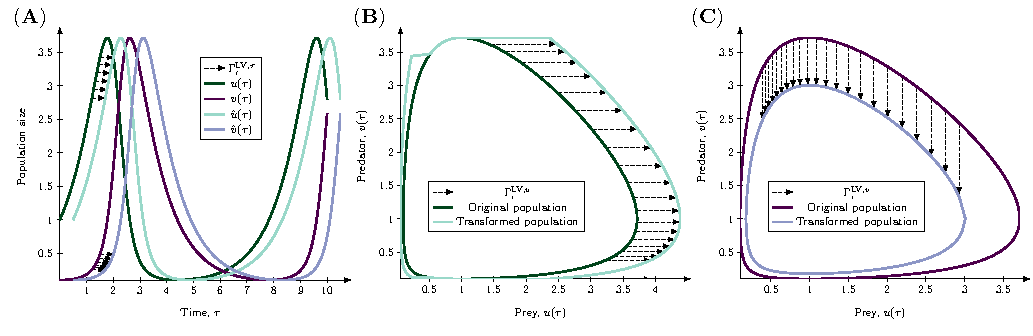
\includegraphics[width=\textwidth]{LV_symmetries}
\caption{\textit{Unidirectional symmetries of the LV-model}. In all cases, the original solution is obtained with the parameter $\alpha=1$, the initial conditions $(u_0,v_0)=(1.00,0.10)$ and the solutions are then transformed with a transformation parameter of $\epsilon=0.5$. (\textbf{A}) The action of the time translation symmetry $\Gamma^{\mathrm{LV},\tau}_{\epsilon}$. (\textbf{B}) The action of the $u$-directional symmetry $\Gamma^{\mathrm{LV},u}_{\epsilon}$. (\textbf{C}) The action of the $v$-directional symmetry $\Gamma^{\mathrm{LV},v}_{\epsilon}$.}
\label{fig:LV_symmetries}
\end{center}
\end{figure}
% --------------------------------------------------------------------------------------
%--------------------------------------------------------------------------------------
% The SIR model
\section{The symmetries of the SIR-model}
We remind ourselves that we want to study the SIR model
\begin{equation*}
  \begin{split}
    \dv{S}{t}&=-rSI,\\
    \dv{I}{t}&=rSI-aI.\\
    \dv{R}{t}&=aI.\\    
    \end{split}
  \end{equation*}
  and we are looking for a generator of the following kind:
\begin{equation}
X=\xi(t,S,I,R)\partial_t+\eta_1(t,S,I,R)\partial_S+\eta_2(t,S,I,R)\partial_I+\eta_3(t,S,I,R)\partial_R.
\end{equation}
\subsection{Ans\"atze assuming that the equations for the tangents are independent of the states}
%--------------------------------------------------------------------------------------
%--------------------------------------------------------------------------------------
% The BZ-model
\section{The symmetries of the BZ-model}
The infinitesimal generators of the Lie group that where found with polynomial ans\"atze of degree $d_3=d_4=5$ for the infinitesimals $\eta_1(u,v)$ and $\eta_2(u,v)$ were the following:


\begin{align*}
X_{1}&=\frac{u \left(u^{3} - 3 u - 3 v\right)}{3 e}\partial_u+u^{2}\partial_v,\\
X_{2}&=\frac{v^{2} \left(u^{3} - 3 u - 3 v\right)}{3 e}\partial_u+u v^{2}\partial_v,\\
X_{3}&=\frac{u v \left(u^{3} - 3 u - 3 v\right)}{3 e}\partial_u+u^{2} v\partial_v,\\
X_{4}&=\frac{u^{3} - 3 u - 3 v}{3 e}\partial_u+u\partial_v,\\
X_{5}&=\frac{v \left(u^{3} - 3 u - 3 v\right)}{3 e}\partial_u+u v\partial_v,\\
X_{6}&=\frac{u^{2} \left(u^{3} - 3 u - 3 v\right)}{3 e}\partial_u+u^{3}\partial_v.\\
\end{align*}


Note that the reaction terms are:

\begin{align*}
\omega_1(u,v)&=\frac{v}{e} - \frac{\frac{u^{3}}{3} - u}{e},\\
\omega_2(u,v)&=- u.\\
\end{align*}


so all these generators are trivial.


% --------------------------------------------------------------------------------------
%--------------------------------------------------------------------------------------
% 
\section{The symmetries of the Brusselator}
We remind ourselves that we want to study the Brusselator model

\begin{equation*}
  \begin{split}
    \dv{u}{t}&=1-(b-1)u+au^2 v,\\
    \dv{v}{t}&=bu-au^2 v.\\
    \end{split}
\end{equation*}
and we are looking for a generator of the following kind:
\begin{equation}
X=\xi(t,u,v)\partial_t+\eta_1(t,u,v)\partial_u+\eta_2(t,u,v)\partial_v.
\end{equation}
Now, the first linearised symmetry condition is
\begin{align}
  - a^{2} u^{4} v^{2} \pdv{\xi}{u} + a^{2} u^{4} v^{2} \pdv{\xi}{v} + 2 a b u^{3} v \pdv{\xi}{u} - 2 a b u^{3} v \pdv{\xi}{v}&\nonumber\\
  - 2 a \eta_1 u v - a \eta_2 u^{2} - 2 a u^{3} v \pdv{\xi}{u} + a u^{3} v \pdv{\xi}{v}&\nonumber\\
  + a u^{2} v \pdv{\eta_1}{u} - a u^{2} v \pdv{\eta_1}{v} - 2 a u^{2} v \pdv{\xi}{u} + a u^{2} v \pdv{\xi}{v}&\nonumber\\
  - a u^{2} v \pdv{\xi}{t} - b^{2} u^{2} \pdv{\xi}{u} + b^{2} u^{2} \pdv{\xi}{v} + b \eta_1&\nonumber\\
  + 2 b u^{2} \pdv{\xi}{u} - b u^{2} \pdv{\xi}{v} - b u \pdv{\eta_1}{u} + b u \pdv{\eta_1}{v} &\nonumber\\
  + 2 b u \pdv{\xi}{u} - b u \pdv{\xi}{v} + b u \pdv{\xi}{t} - \eta_1&\nonumber\\
  - u^{2} \pdv{\xi}{u} + u \pdv{\eta_1}{u} - 2 u \pdv{\xi}{u} - u \pdv{\xi}{t} + \pdv{\eta_1}{u}&\nonumber\\
  - \pdv{\xi}{u} + \pdv{\eta_1}{t} - \pdv{\xi}{t}&=0,\label{eq:Brusselator_lin_sym_1}
\end{align}
while the second linearised symmetry condition is given by
\begin{align}
  a^{2} u^{4} v^{2} \pdv{\xi}{u} - a^{2} u^{4} v^{2} \pdv{\xi}{v} - 2 a b u^{3} v \pdv{\xi}{u} + 2 a b u^{3} v \pdv{\xi}{v}&\nonumber\\
  + 2 a \eta_1 u v + a \eta_2 u^{2} + a u^{3} v \pdv{\xi}{u} + a u^{2} v \pdv{\eta_2}{u}&\nonumber\\
  - a u^{2} v \pdv{\eta_2}{v} + a u^{2} v \pdv{\xi}{u} + a u^{2} v \pdv{\xi}{t} + b^{2} u^{2} \pdv{\xi}{u}&\nonumber\\
  - b^{2} u^{2} \pdv{\xi}{v} - b \eta_1 - b u^{2} \pdv{\xi}{u} - b u \pdv{\eta_2}{u}&\nonumber\\
  + b u \pdv{\eta_2}{v} - b u \pdv{\xi}{u} - b u \pdv{\xi}{t} + u \pdv{\eta_2}{u}&\nonumber\\
  + \pdv{\eta_2}{u} + \pdv{\eta_2}{t}&=0.\label{eq:Brusselator_lin_sym_2}
\end{align}


\subsection{Ans\"atze assuming that the equations for the tangents are independent of the states}
Again, the assumption that the derivatives of the tangents are at most functions of the time $t$ amounts to finding the roots of a polynomial of the states $u$ and $v$. Since these monomials are linearly independent we obtain the following equations:
\begin{align}
1:&b \eta_1 - \eta_1 + \pdv{\eta_1}{u} - \pdv{\xi}{u} + \pdv{\eta_1}{t} - \pdv{\xi}{t}=0\\
u:&- b \pdv{\eta_1}{u} + b \pdv{\eta_1}{v} + 2 b \pdv{\xi}{u} - b \pdv{\xi}{v} + b \pdv{\xi}{t} + \pdv{\eta_1}{u} - 2 \pdv{\xi}{u} - \pdv{\xi}{t}=0\\
u v:&- 2 a \eta_1=0\\
u^{2}:&- a \eta_2 - b^{2} \pdv{\xi}{u} + b^{2} \pdv{\xi}{v} + 2 b \pdv{\xi}{u} - b \pdv{\xi}{v} - \pdv{\xi}{u}=0\\
u^{2} v:&a \pdv{\eta_1}{u} - a \pdv{\eta_1}{v} - 2 a \pdv{\xi}{u} + a \pdv{\xi}{v} - a \pdv{\xi}{t}=0\\
u^{3} v:&2 a b \pdv{\xi}{u} - 2 a b \pdv{\xi}{v} - 2 a \pdv{\xi}{u} + a \pdv{\xi}{v}=0\\
u^{4} v^{2}:&- a^{2} \pdv{\xi}{u} + a^{2} \pdv{\xi}{v}=0,
\end{align}
for the first linearised symmetry condition and the following equations
\begin{align}
1:&- b \eta_1 + \pdv{\eta_2}{u} + \pdv{\eta_2}{t}=0\\
u:&- b \pdv{\eta_2}{u} + b \pdv{\eta_2}{v} - b \pdv{\xi}{u} - b \pdv{\xi}{t} + \pdv{\eta_2}{u}=0\\
u v:&2 a \eta_1=0\\
u^{2}:&a \eta_2 + b^{2} \pdv{\xi}{u} - b^{2} \pdv{\xi}{v} - b \pdv{\xi}{u}=0\\
u^{2} v:&a \pdv{\eta_2}{u} - a \pdv{\eta_2}{v} + a \pdv{\xi}{u} + a \pdv{\xi}{t}=0\\
u^{3} v:&- 2 a b \pdv{\xi}{u} + 2 a b \pdv{\xi}{v} + a \pdv{\xi}{u}=0\\
u^{4} v^{2}:&a^{2} \pdv{\xi}{u} - a^{2} \pdv{\xi}{v}=0,
\end{align}
for the second linearised symmetry condition.
%--------------------------------------------------------------------------------------
% THE BIBLIOGRAPHY
%--------------------------------------------------------------------------------------
\clearpage
\bibliographystyle{unsrt}
\bibliography{symmetry_bib}
%--------------------------------------------------------------------------------------
% THE DOCUMENT ENDS
%--------------------------------------------------------------------------------------
\end{document}